\section{Result}
\begin{figure}[H]
\centering
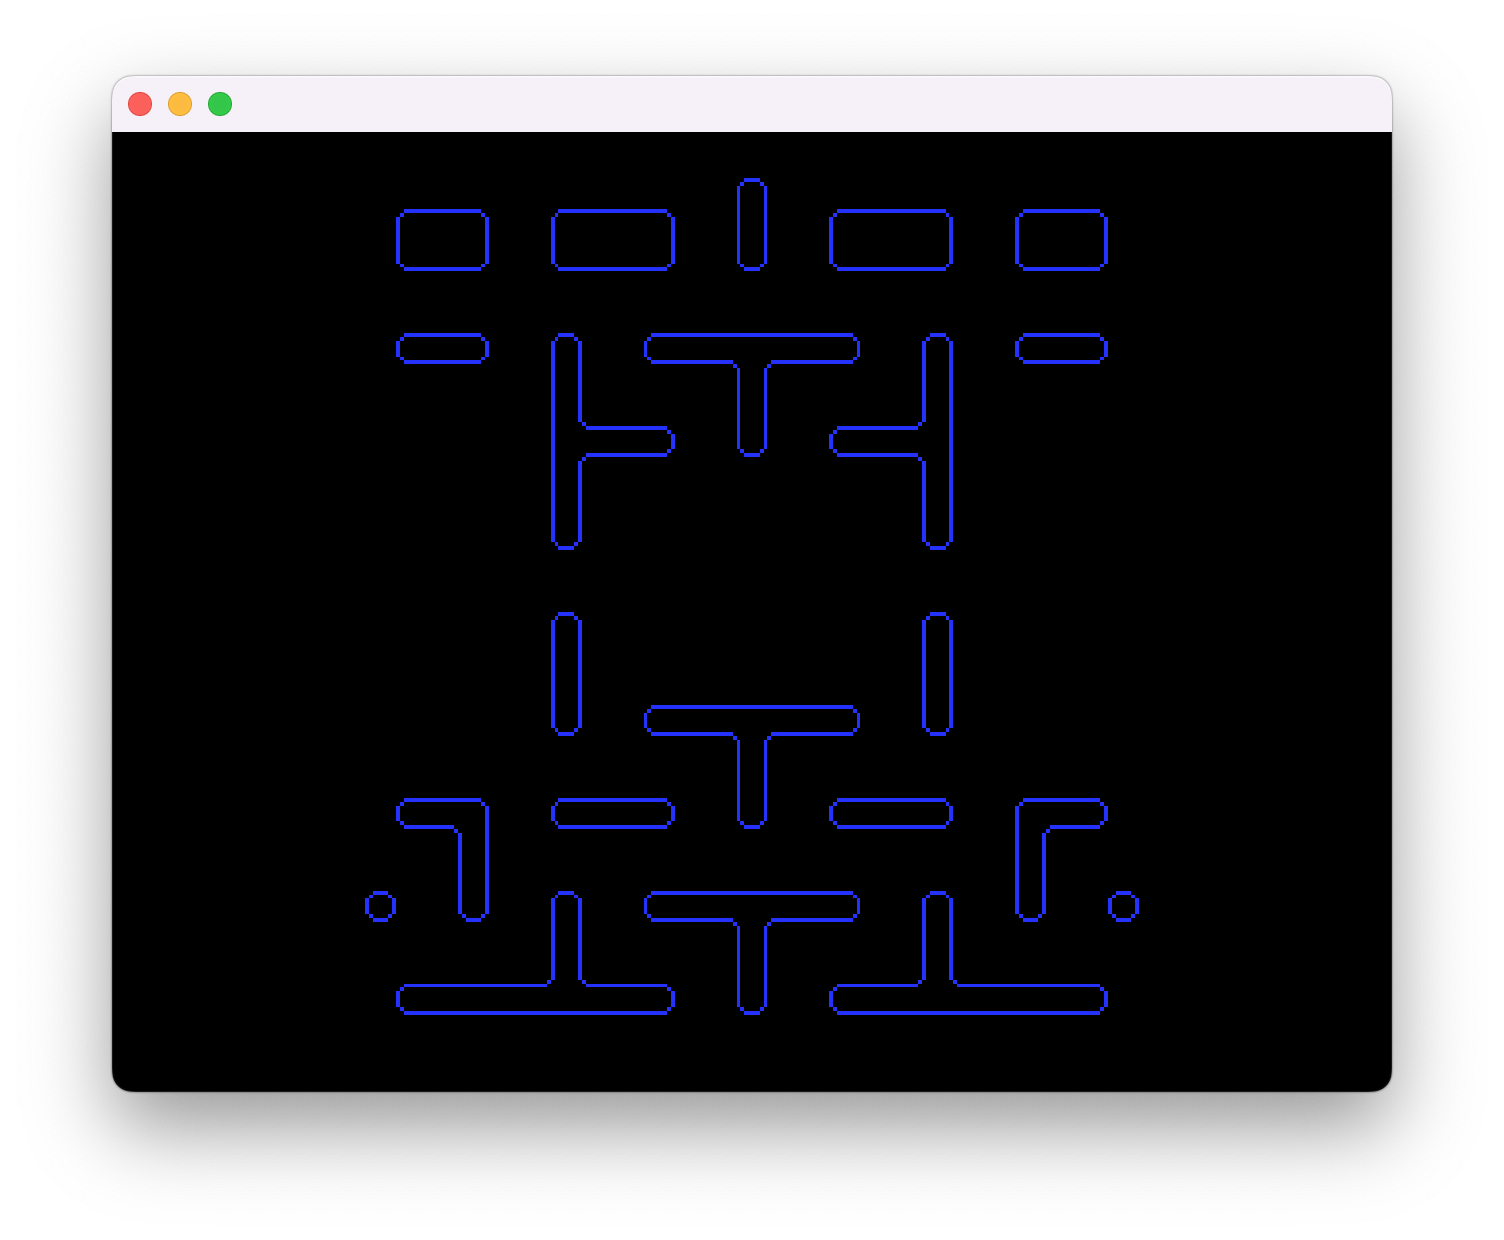
\includegraphics[width=0.8\linewidth]{Image-8.png}
\caption {Output of first algorithm\autocite{myself}}\label{FirstOutput}
\end{figure}

\section{Analysis of Algorithm 1}
Algorithms run at speeds related to the number of operations that they must make, based on the input size. This is described by the big-O notation $O(f(x))$ where $f(x)$ is a function relating the input size to the steps the algorithm must make. Our algorithm, applied to a square lattice graph of a boundary customary to Pac-Man will step on each tile exactly once, and at each tile will check at most 3 directions (all cardinal directions except for the one we walked from). Thus if we let the input size $n$ be the number of tiles in a wall boundary, then we have a speed of $O(3n)$, also refered to as linear-time complexity, meaning that as the input size increases linearly, the time taken by the algorithm will, in the worst case, change proportionally to that, which is considered efficient. 

\section{Limitations of Algorithm 1}
Figure~\ref{FirstOutput}, shows the algorithm applied to the original Pac-Man level. Most of the tiles are colored, yet the image is missing the tiles forming the boundary of the level, when comparing with Figure~\ref{PacmanLevelGrid}. This is because the outer boundary is fundamentally different from the central ones in structure, we can see the isolated outer boundary in Figure~\ref{OuterBoundary}.
\begin{figure}[H]
\centering
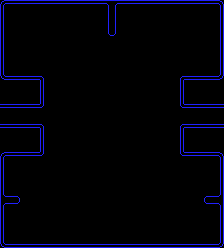
\includegraphics[width=0.6\linewidth]{Image-11.png}
\caption {Outer boundary that cannot be produced with algorithm 1.\autocite{pittman_pac-man_2009}}\label{OuterBoundary}
\end{figure}
\section{Differences between the Outer Boundary and the Inner Boundaries}
\begin{enumerate}
\item { \bf The geometry of the Pac-Man plane.} There appear two gaps to the east and west of the outer boundary. In the game, Pac-Man can move into one of these gaps and appear on the other side. Thus the Pac-Man level, although previously assumed to be a Euclidean plane, extending infinitely in all directions with each point described by a unique pair of integers, can be better described as a curved surface, revolving around itself horizontally by the width of the level. We can extend this definition by assuming a vertical revolution by the height of the level as well. Thus any integer coordinate $(x,y)$ must appear in our context as $(x \pmod{width}, y\pmod{height})$. As per this definition, we can shift the appearance of the outer boundary on the curved surface, maintaining its structure as seen in Figure~\ref{ShiftedOuterBoundary}.
\begin{figure}[H]
\centering
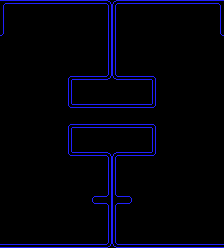
\includegraphics[width=0.6\linewidth]{Image-12.png}
\caption {Outer boundary shifted by the half of the width of the level.\autocite{pittman_pac-man_2009}}\label{ShiftedOuterBoundary}
\end{figure}
This makes Lemma~\ref{NorthwestCornerLemma} redundant, which assumed that there must be a westernmost vertex out of northernmost vertices. In a curved surface the concept of westernmost and northernmost do not exist without a clear reference point, as we can move in any cardinal direction and come back to the same point we started from. 
\item {\bf The normal function according to which we turn in our algorithm walking the Hamiltonian cycle.} If we assume the gaps in the outer boundary to be filled in with straight walls connecting the two halves into a single outer boundary, and ignore the geometry of the level, the normal function is reversed. Instead of $Normal(d)=d+1\pmod{4}$ we get $Normal'(d)=d+3\pmod{4}$. Instead of turning "outwards" we turn "inwards". This is illustrated in Figure~\ref{ConnectedOuterBoundary}. 
\begin{figure}[H]
\centering
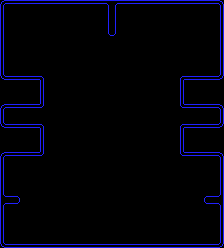
\includegraphics[width=0.6\linewidth]{Image-13.png}
\caption {Outer boundary connected in the gaps, showing a deviation from our previously defined normal function.\autocite{pittman_pac-man_2009}}\label{ConnectedOuterBoundary}
\end{figure}
\end{enumerate}
